\documentclass[12pt, a4paper]{article}
\usepackage[T2A]{fontenc}
\usepackage[utf8]{inputenc}
\usepackage[russian]{babel}
\usepackage{graphicx}
\usepackage{amsfonts}
\usepackage{indentfirst}
\usepackage{amsmath}
\usepackage{amsthm}
\usepackage{nicematrix}
\usepackage{hyperref}
\hypersetup{
    colorlinks=true,
    linkcolor=black,
    filecolor=magenta,      
    urlcolor=cyan,
    pdftitle={Lab4},
    pdfpagemode=FullScreen,
}
\usepackage{soulutf8}
\usepackage[left=1cm,right=1cm,
    top=2cm,bottom=2cm]{geometry}
\usepackage{titleps}
    \newpagestyle{main}{
        \setheadrule{0.4pt}
        \sethead{something}{\thepage}{}
}
\usepackage{listings}
\usepackage{color}

\definecolor{dkgreen}{rgb}{0,0.6,0}
\definecolor{gray}{rgb}{0.5,0.5,0.5}
\definecolor{mauve}{rgb}{0.58,0,0.82}

\lstset{frame=tb,
  language=Python,
  aboveskip=3mm,
  belowskip=3mm,
  showstringspaces=false,
  columns=flexible,
  basicstyle={\small\ttfamily},
  numbers=none,
  numberstyle=\tiny\color{gray},
  keywordstyle=\color{blue},
  commentstyle=\color{dkgreen},
  stringstyle=\color{mauve},
  breaklines=true,
  breakatwhitespace=true,
  tabsize=3
}
%\pagestyle{main}
\theoremstyle{plain}
\newtheorem{theorem}{Теорема}[section]
\newtheorem{corollary}{Следствие}[theorem]
\newtheorem*{example}{\textit{Пример}}
\newtheorem*{definition}{Определение}

\begin{document}
\begin{titlepage}
  \newpage
  \begin{center}
  \begin{tabular}{cc}
       \parbox{12cm}{\centering \textbf{НИУ ИТМО}}\\
       \\
       \hline
       \hline
  \end{tabular}
  \end{center}

  \begin{center}
  \caps{\textbf{Факультет систем управления и робототехники}}\\ 
  \end{center}
  
  \vspace{1cm}
  
  \begin{center}
      \textsc{Лабораторная работа № 3\\ по дисциплине <<Частотные методы>>}
  \end{center}
  
  \vspace{8em}
  
  \noindent Выполнил:  \hfill Гридусов Д.Д
  
  \vspace{20pt}
  \noindent Преподаватель: \hfill Перегудин А.А \\
  \\
  \vfill
  \begin{center}
  Санкт-Петербург \\2024 г.
  \end{center}
  
  \end{titlepage}
  
  \tableofcontents
  \newpage
  \section{Жёсткая фильтрация}
  \subsection{Убираем высокие частоты}
  \noindent Для начала нарисуем график исходной ситуации для случая $c = 0$, $a = 2$, $b = 0.32$ и попытаемся убрать высокие частоты с помощью преборазования Фурье.
  \begin{figure}[!h]
    \centering
    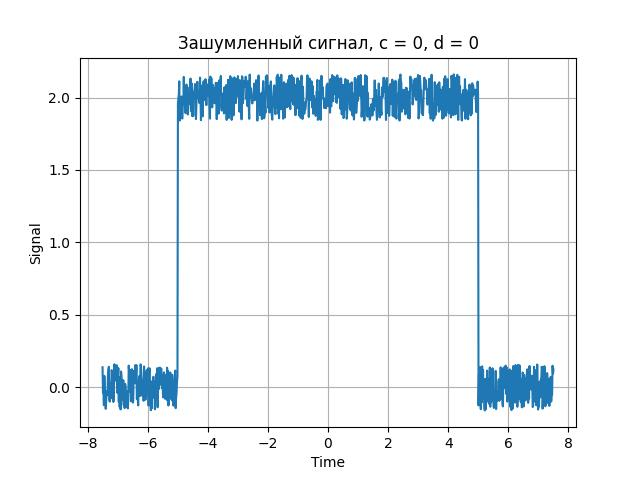
\includegraphics[scale=0.78]{../images/result/original_s1.jpeg}
    \caption{Зашумленный сигнал c = 0, d = 0}
  \end{figure}
  \begin{figure}[!h]
    \centering
    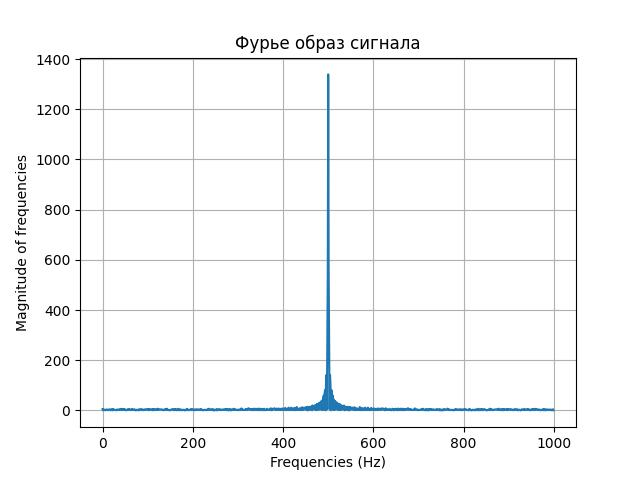
\includegraphics[scale=0.78]{../images/result/original_s1_fourier.jpeg}
    \caption{Фурье-образ}
  \end{figure}
  \\
  \noindent Сразу обратим внимание на то, что параметр $b$ отвечает за степень зашумленности сигнала - покажем это на графике.
  \begin{figure}[!h]
    \centering
    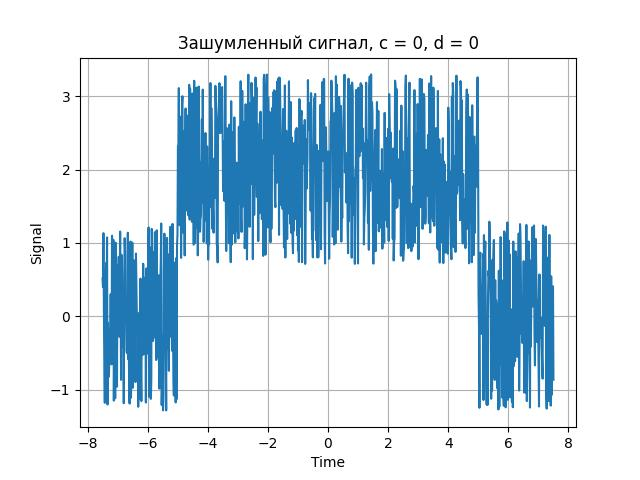
\includegraphics[scale=0.78]{../images/result/original_s2.jpeg}
    \caption{Зашумленный сигнал с большим параметром b}
  \end{figure}
  \begin{figure}[!h]
    \centering
    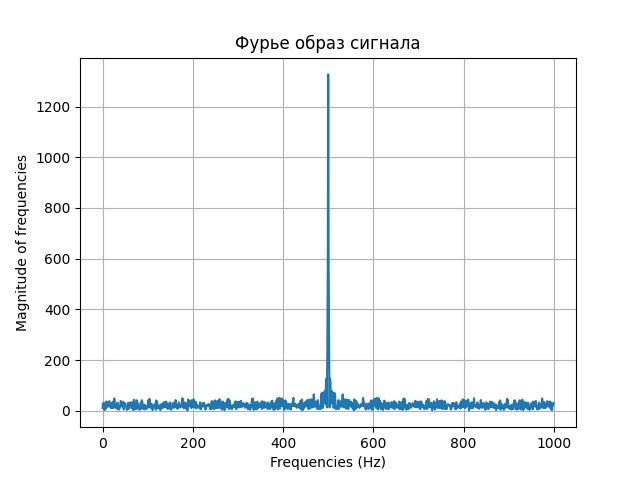
\includegraphics[scale=0.78]{../images/result/original_s2_fourier.jpeg}
    \caption{Фурье-образ более зашумленного сигнала}
  \end{figure}
  \\
  \noindent Напишем функцию для фильтрации верхних частот
  \\
  \textbf{Листинг 1.1} Фильтрация верхних частот
  \begin{lstlisting}
  # Filter that removes only some high frequencies from signal
  def high_freq_filtration(fourier_image, treshold):
      n = fourier_image.shape[0]
      frequencies_range = np.linspace(-n/2, n/2, 1000)
      counter = 0
      for k in frequencies_range:
          if (abs(k) >= treshold):
              fourier_image[counter] = 0
          counter += 1
      return fourier_image
  \end{lstlisting}
  \noindent Применим фильтры к обоим сигналам.
  \begin{figure}[!htb]
    \minipage{0.5\textwidth}
      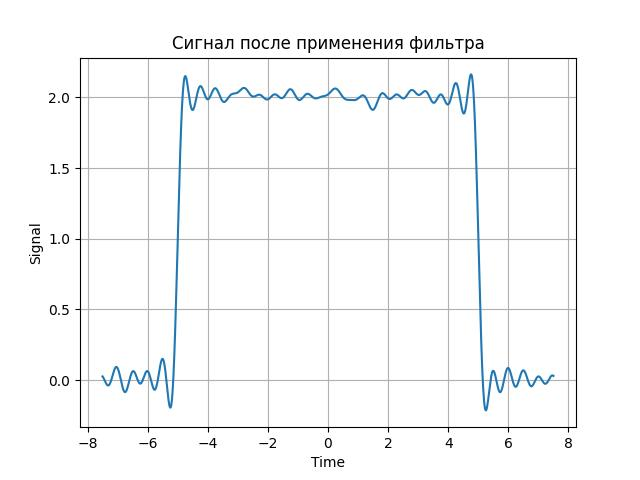
\includegraphics[width=\linewidth]{../images/result/high_freq1.jpeg}
      \caption{Фильтрация первого сигнала с $b = 0.32$}
    \endminipage\hfill
    \minipage{0.5\textwidth}
      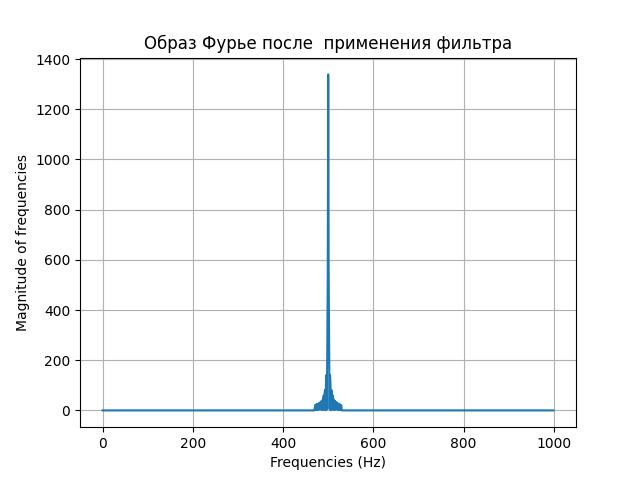
\includegraphics[width=\linewidth]{../images/result/high_freq1_fourier.jpeg}
      \caption{Фурье-образ первого сигнала}
    \endminipage\hfill
    \end{figure}

    \begin{figure}[!htb]
      \minipage{0.5\textwidth}
        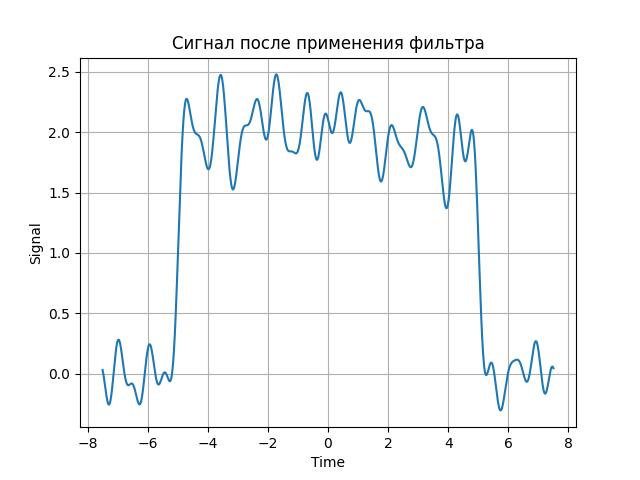
\includegraphics[width=\linewidth]{../images/result/high_freq2.jpeg}
        \caption{Фильтрация второго сигнала с $b = 2.6$}
      \endminipage\hfill
      \minipage{0.5\textwidth}
        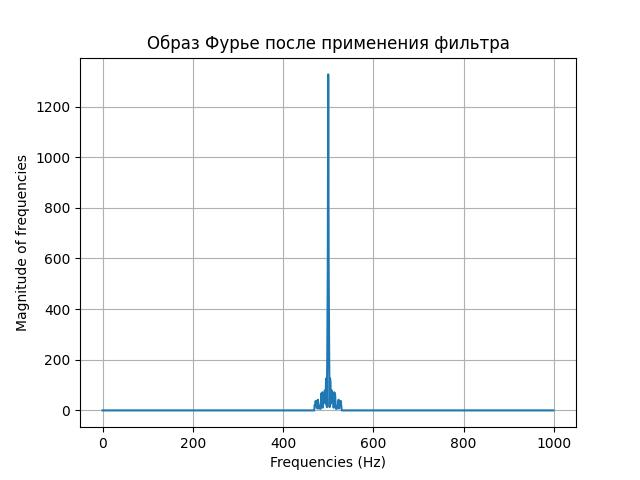
\includegraphics[width=\linewidth]{../images/result/high_freq2_fourier.jpeg}
        \caption{Фурье-образ второго сигнала}
      \endminipage\hfill
      \end{figure}

    \noindent Со вторым сигналам получилось гораздо хуже, что можно было предположить, так как чем больше шума, тем сложнее от него избавиться.
    \subsection{Убираем специфические частоты}
    \noindent В этом задании у сигнала появиться еще и сдвиг на фазу, но (хоть я и не сразу это понял), получить после фильтрации нужно исходную прямоугольную волну. Империческое наблюдение - чем шире исходная квадртаная волна, тем сильнее она отличается от синусоидальной функции и тем проще фильтру восстановить исходный сигнал.
    \begin{figure}[!htb]
      \minipage{0.5\textwidth}
        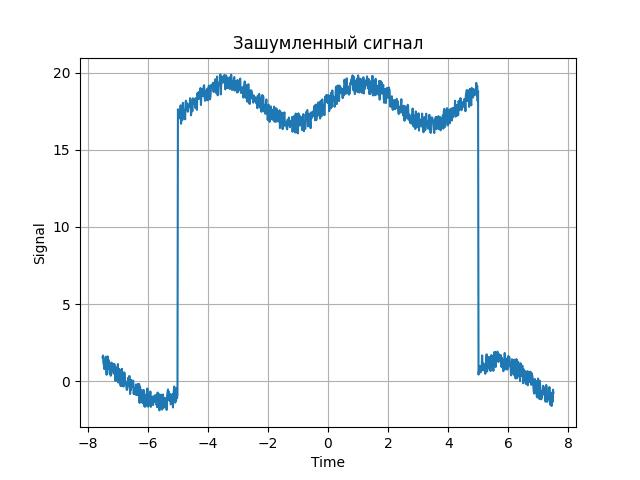
\includegraphics[width=\linewidth]{../images/result/orginal_s3.jpeg}
        \caption{Зашумленный сигнал + сдвиг на фазу}
      \endminipage\hfill
      \minipage{0.5\textwidth}
        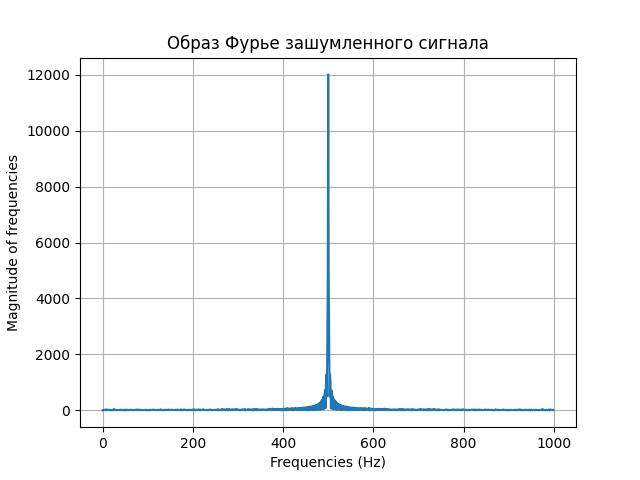
\includegraphics[width=\linewidth]{../images/result/original_s3_fourier.jpeg}
        \caption{Фурье-образ}
      \endminipage\hfill
      \end{figure}
      \begin{figure}[!htb]
        \minipage{0.5\textwidth}
          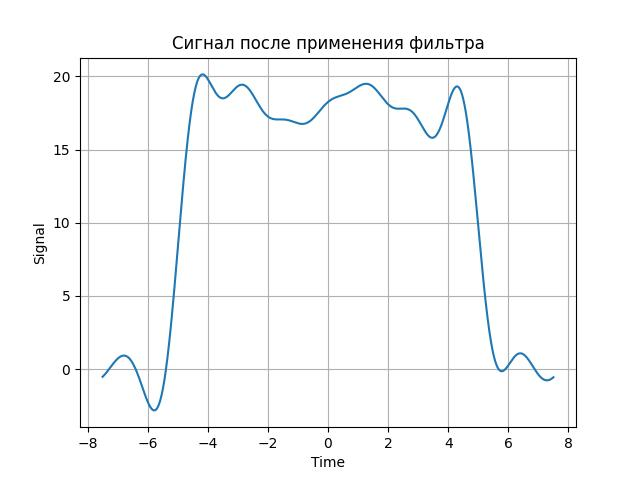
\includegraphics[width=\linewidth]{../images/result/spec_freq.jpeg}
          \caption{Фильтрация шума и сдвига}
        \endminipage\hfill
        \minipage{0.5\textwidth}
          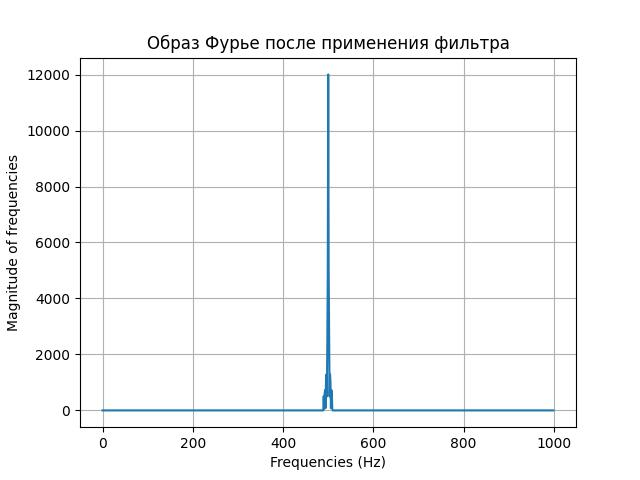
\includegraphics[width=\linewidth]{../images/result/spec_freq_fourier.jpeg}
          \caption{Фурье-образ отфильтрованного сигнала}
        \endminipage\hfill
        \end{figure}
        \\
        \noindent Заметно, что фильтр справляется достаточно неплохо, но что будет если убрать шум и оставить только сдвиг на фазу? Положим $b = 0$:
       \newpage
        \begin{figure}[!htb]
          \minipage{0.5\textwidth}
            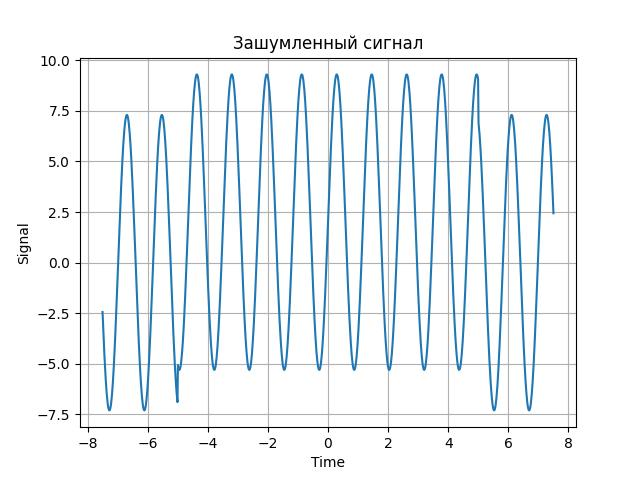
\includegraphics[width=\linewidth]{../images/result/orginal4.jpeg}
            \caption{$b = 0$ и сдвиг на фазу}
          \endminipage\hfill
          \minipage{0.5\textwidth}
            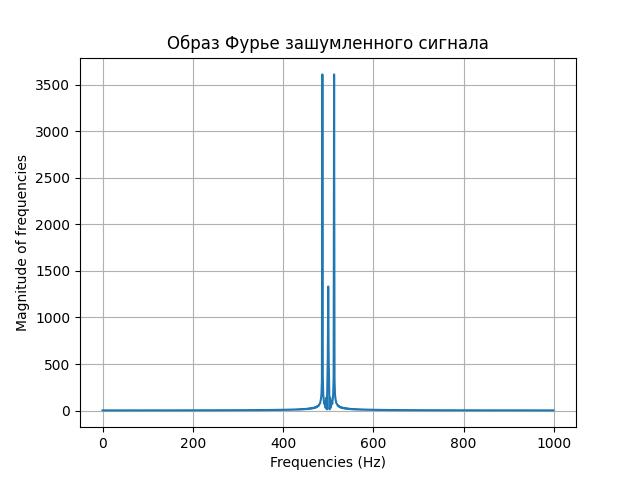
\includegraphics[width=\linewidth]{../images/result/original4_fourier.jpeg}
            \caption{Фурье-образ}
          \endminipage\hfill
          \end{figure}
          \begin{figure}[!htb]
            \minipage{0.5\textwidth}
              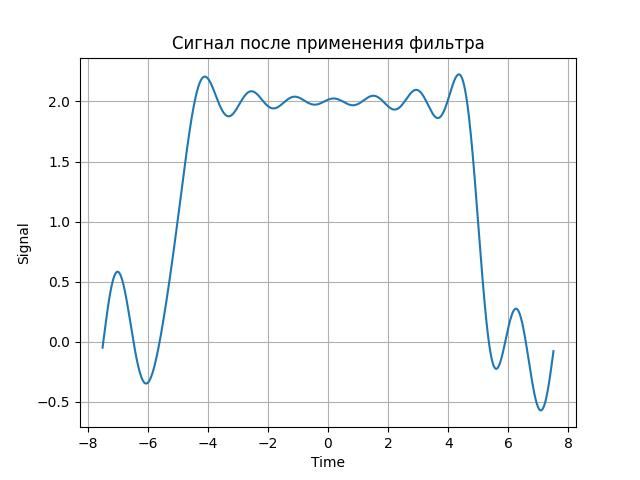
\includegraphics[width=\linewidth]{../images/result/spec_freq2.jpeg}
              \caption{Результат фильтрации}
            \endminipage\hfill
            \minipage{0.5\textwidth}
              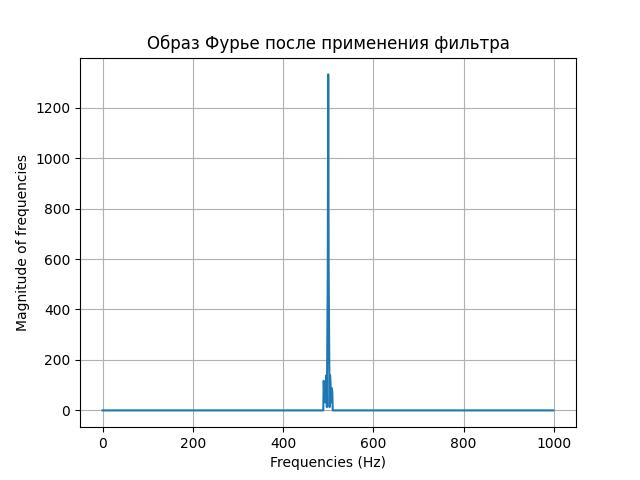
\includegraphics[width=\linewidth]{../images/result/spec_freq2_fourier.jpeg}
              \caption{Фурье-образ отфильтрованного сигнала}
            \endminipage\hfill
            \end{figure}
        \noindent Восстановленный сигнал очень похож на квадратную волну, что не может не радовать. 
        \\
        \noindent \textbf{Листинг 1.2} Фильтрация специфических частот
        \begin{lstlisting}
  # Filter that will remove both high and low freqs
  def spec_freq_filtration(fourier_image, treshold1, treshold2):
    n = fourier_image.shape[0]
    frequencies_range = np.linspace(-n/2, n/2, 1000)
    counter = 0 
    for k in frequencies_range:
      if (abs(k) <= treshold1) or (abs(k) >= treshold2):
        fourier_image[counter] = 0
        counter += 1
    return fourier_image
        \end{lstlisting}
        
       \newpage 
   \subsection{Фильтрация нижних частот}
   \noindent \textbf{Листинг 1.3} Фильтрация нижних частот
        \begin{lstlisting}
  # Filter that will remove only some low freqs
  def low_freq_filtration(fourier_image, treshold1):
    n = fourier_image.shape[0]
    frequencies_range = np.linspace(-n/2, n/2, 1000)
    counter = 0
    for k in frequencies_range:
      if (abs(k) <= treshold1):
        fourier_image[counter] = 0
        counter += 1
    return fourier_image
        \end{lstlisting}
   \begin{figure}[!htb]
    \minipage{0.5\textwidth}
      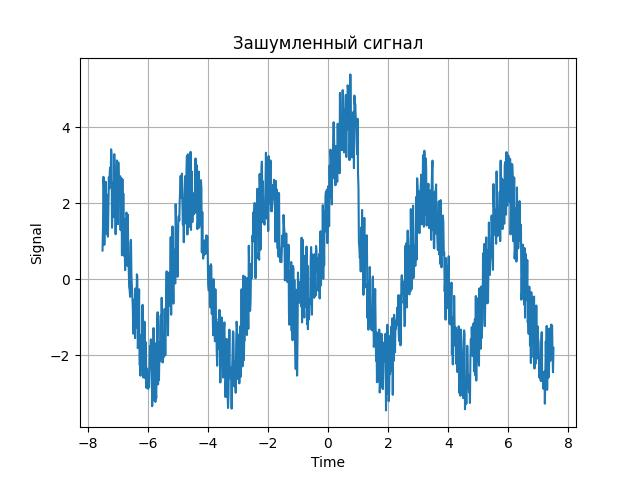
\includegraphics[width=\linewidth]{../images/result/original_s5.jpeg}
      \caption{Зашумленный сигнал + сдвиг, все параметры больше 0}
    \endminipage\hfill
    \minipage{0.5\textwidth}
      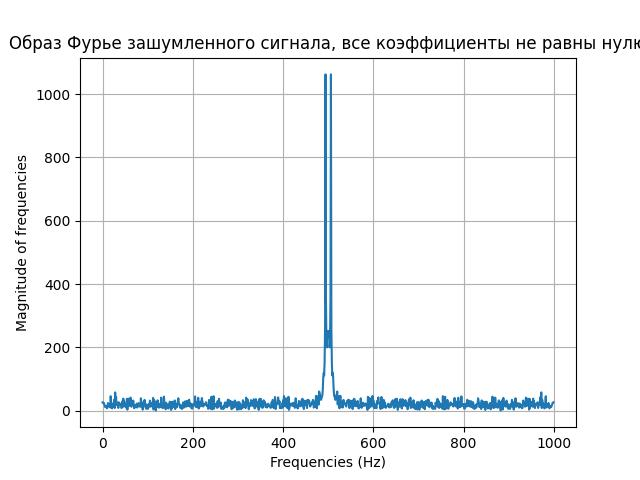
\includegraphics[width=\linewidth]{../images/result/original_s5_fourier.jpeg}
      \caption{Фурье-образ}
    \endminipage\hfill
    \end{figure}
    \noindent Исходя из логики предыдщего пункта, чтобы убрать шум и сдвиг, нам нужно обнулить нехарактерные исходному сигналу два "горба" у образа Фурье, оставив при этом частоты, находящиеся между этими горбами. Но, как будет видно и по графику, это не получается сделать при любом диапазоне запретных частот.
    
    \clearpage
    \begin{figure}[!htb]
      \minipage{0.5\textwidth}
        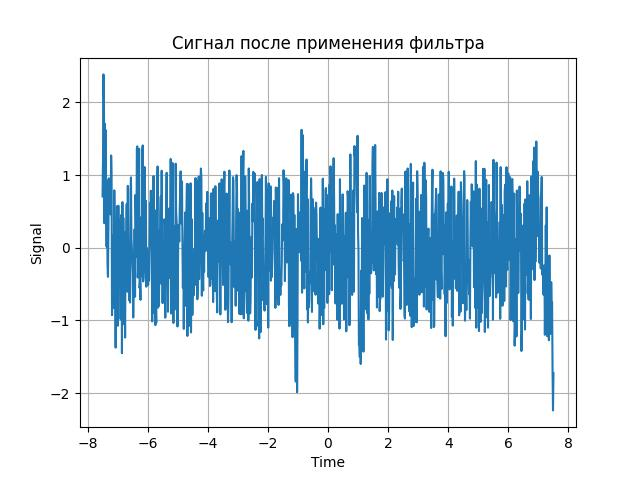
\includegraphics[width=\linewidth]{../images/result/low_freq.jpeg}
        \caption{Результат фильтрации}
      \endminipage\hfill
      \minipage{0.5\textwidth}
        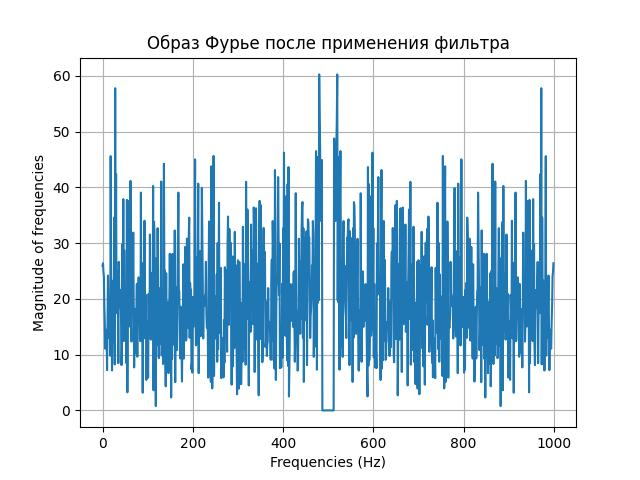
\includegraphics[width=\linewidth]{../images/result/low_freq_fourier.jpeg}
        \caption{Фурье-образ отфильтрованного сигнала}
      \endminipage\hfill
      \end{figure}
      \noindent Видно, что фильтрации не получилось.

      \section{Фильтрация звука}
      Сначала прочитаем звуковую волну из .wav файла и построим 
      ее образ Фурье:
      \begin{figure}[!htb]
        \minipage{0.5\textwidth}
          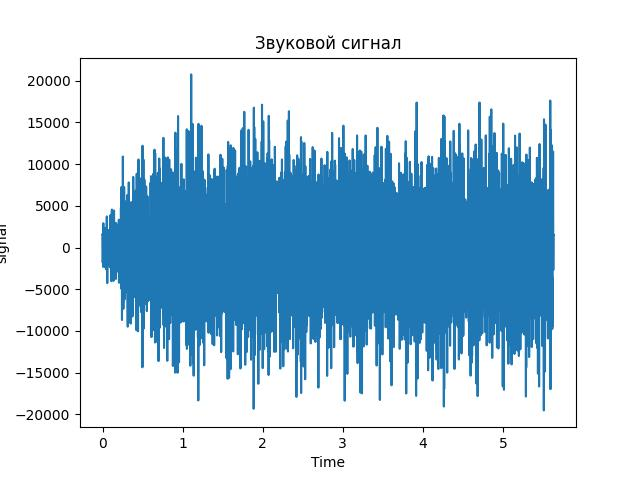
\includegraphics[width=\linewidth]{../images/result/sound_wave.jpeg}
          \caption{Зашумленная звуковая волна}
        \endminipage\hfill
        \minipage{0.5\textwidth}
          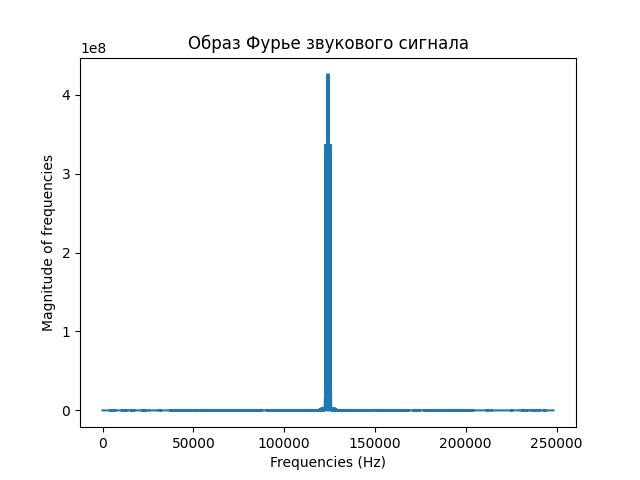
\includegraphics[width=\linewidth]{../images/result/soundwave_fourier.jpeg}
          \caption{Фурье-образ исходной звуковой волны}
        \endminipage\hfill
        \end{figure}
        \noindent Судя по распределению частот  лучше всего будет убирать высокие частоты, так мы и сделаем.
        
       \newpage
          \begin{figure}[!htb]
            \minipage{0.5\textwidth}
              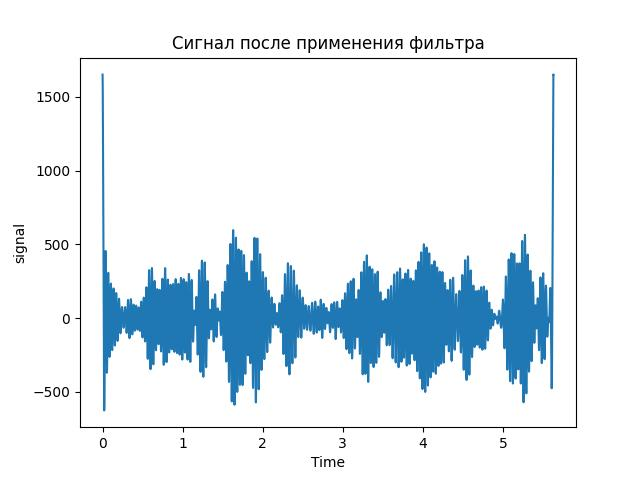
\includegraphics[width=\linewidth]{../images/result/soundwave_filtration1.jpeg}
              \caption{Звуковая волна после фильтра.}
            \endminipage\hfill
            \minipage{0.5\textwidth}
              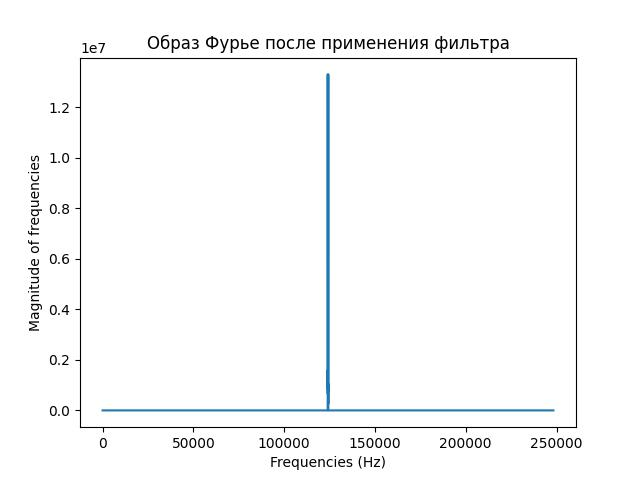
\includegraphics[width=\linewidth]{../images/result/soundwave_filtration1_fourier.jpeg}
              \caption{Фурье-образ отфильтрованного сигнала}
            \endminipage\hfill
            \end{figure}
            \noindent \textbf{Вывод: } заметно, что фильтр помог и остался только содержательный звук
    \section{Исходный код на github}
   \noindent Весь код лабораторной работы №3: \href{https://github.com/D2J3D/Fourier_Labs/tree/main}{исходники}
            \end{document}